\documentclass{article} % For LaTeX2e
\usepackage{cos424,times}
\usepackage{url}
\usepackage{graphicx}
\usepackage{hyperref}
\usepackage{amsmath}

\title{Sentiment analysis of online reviews}


\author{
	Charles Stahl\\
	Department of Physics\\
	Princeton University\\
	\texttt{cnstahl@} \\
	\And
	Meir Hirsch \\
	Department of Computer Science\\
	Princeton University \\
	\texttt{ehirsch@} \\
}

\newcommand{\fix}{\marginpar{FIX}}
\newcommand{\new}{\marginpar{NEW}}

\begin{document}
	
	\maketitle
	
	\begin{abstract}
		With the proliferation of short text snippets on the Internet, especially in social networks, there is a growing need to be able to classify these texts with very little context. This can be as simple as classifying snippets as positive or negative. One place where this would be helpful is in online reviews, so that sellers can gauge the reaction through a metric separate from number-of-stars reviews. On social media, one might want to look at all mentions of a person or hashtag and see whether general sentiment is positive or negative.
	\end{abstract}
	
	\section{Introduction}
	
	With the proliferation of short text snippets on the Internet, especially in social networks, there is a growing need to be able to classify these texts with very little context. This can be as simple as classifying snippets as positive or negative. One place where this would be helpful is in online reviews, so that sellers can gauge the reaction through a metric separate from number-of-stars reviews. On social media, one might want to look at all mentions of a person or hashtag and see whether general sentiment is positive or negative.
	
	In this paper, we evaluate {\bf some methods} in their ability to classify the sentiments of online reviews as either positive or negative. We evaluate from the perspective of looking for negative reviews or looking for positive reviews. We evaluate the methods using a simple bag-of-words representation with and without feature selection. 
	
	Such a sentiment classifier could conceivably be useful to producers and consumers. Producers would want to find the negative reviews in order to know what they most need to improve in their products. Consumers could use it to find the products with the most positive reviews.
	
	\section{Related Work}
	
	The data set consists of 2400 training sentences taken from Amazon, Yelp, and iMDB, preprocessed into separate lines and labeled with sentiment. There are also 600 labeled training sentences formatted the same way. The dataset was created by Kotzias et. al. \cite{Kotzias2015}, who analyzed the data using a sentence-level classification method. The optimal accuracy reported in their paper is between 86.0\% and 88.2\%. Preprocessing of the dataset on our end was done in part using the NLTK Python Libraries \cite{nltk}.
	
	The na\"ive attempts in our paper come from the discussion on text classification in Kevin Murphey's \emph{Machine Learning: A Probabilistic Perspective} \cite{Murphy2012}. Specifically, he first suggests using a Bernoulli na\"ive Bayes, then improving upon that with mulinomial na\"ive Bayes (MNB) model. We took the MNB as our starting point. 
	
	
	\section{Methods}
	
	We used the following classification methods
	
	\begin{tabular}{rl}
		a) & Multinomial Na\"ive Bayes\\
	\end{tabular}
	
	All methods we used were implemented using the SciKit Learn Python libraries \cite{scikit-learn}. 
	
	\subsection{Generative vs. Discriminative}
	
	The classifiers we used can be split into two main groups: generative and discriminative classifiers. Generative classifiers are ones that assume a model for the observed features based on the class and then fit the parameters of that model to the training data. This is equivalent to the independence assumption
	\begin{align}
	p(x,z) = p(z)p(x|z),
	\end{align}
	where $x$ is the observation and $z$ is the label. This performs well on small training sets because the assumptions about the model provide a scaffold to build the model on. However, as the training set grows, those assumptions start to hold the classifier back.
	
	Discriminative classifiers, on the other hand, make opposite assumptions. They assume nothing about the distribution of the features given the label, but rather find hypervolumes in the feature space which correspond to a given class. The independence assumtion can be written as 
	\begin{align}
	p(x,z) = p(z|x)p(x).
	\end{align}
	Unlike the generative classifiers, these perform poorly with little data, but improve more with large training sets. 
	
	A disadvantage is that while generative models can trivially handle missing data (one feature not observed for a given sample), discriminative models cannot. This is because a sample missing one feature no longer exists in the full feature space.
	
	\subsection{Feature Extraction and Selection}
	
	Feature extraction was performed during the training portion of the project. One feature used was categorical proportional difference \cite{oKeefe2009}, defined in terms of positive document frequency ($pdf$) and negative document frequency ($ndf$)
	\begin{equation}
	\mbox{CPD} = \frac{|pdf - ndf|}{pdf + ndf},
	\end{equation}
	where the denominator is equivalent to the total number of occurrences of the term in the whole document. Thresholds for both total document frequency and CPD score were set using 5-fold cross-validation.
	
	\subsection{Spotlight on Multinomial Na\"ive Bayes}
	
	The na\"ive Bayes algorithm rests on the assumption of class-conditional independence. The graphical model corresponding to this assumption with $n$ samples and $K$ parameters can be seen in figure \ref{fig:dag}. This figure is taken from a slide in Barbara Engelhardt's lecture on classification \cite{engelhardt17}.
	
	\begin{figure}[h]
		\centering
		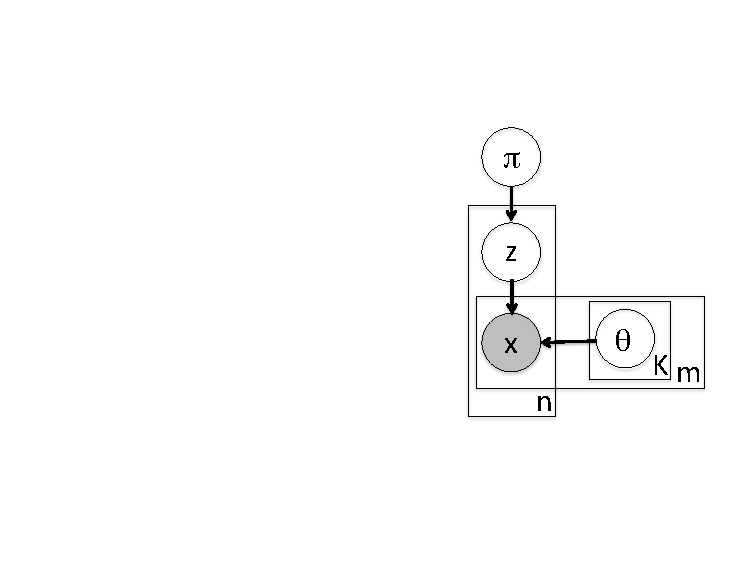
\includegraphics[scale=1]{DAG}
		\caption{The graphical model corresponding to the assumptions of Na\"ive Bayes. The top circle represents the proportion of positive sentiments. $K$ is the number of classes, each with its own parameters, while $n$ is the number of samples. In our case, $\bf x$ is a vector of $m$ features.}
		\label{fig:dag}
	\end{figure}
	
	In the model, $\pi$ is the proportion of samples with positive sentiment. In this case $\pi = .5$. The variable $Z$ is the label of a given sample, i.e. whether the sample is positive or negative. ${\bf x}_i$ is the observed feature vector. When we only use the bag-of-words representation, the features are just the counts of each word. However, when using feature selection, {\bf x} would include those features we selected.
	
	The letter $n$ indicates the number of samples observed. $K$ is the number of classes. $\Theta$ lies inside the $K$ plate because each class has its own probabilities. The last letter, $m$, corresponds to number of features observed. 
	
	The class-conditional independence assumption can be seen in the graph. Once $z_i$ is observed, all components of $\bf x_i$ are independent. Dropping the subscript $i$ corresponding to a single observation and now subscripting w.r.t. components of the feature vector, this can be written as 
	\begin{equation}
	P(x_i|z, x_1,\dots,x_{i-1}, x_{i+1}, \dots, x_m) = P(x_i|z).
	\end{equation}
	This simplifies $P(z|{\bf x})$ as follows:
	\begin{align}
	P(z|{\bf x}) &= \frac{P(z)P({\bf x}|z)}{P({\bf x})} \nonumber\\
	&\propto P(z)\sum_{i=1}^mP(x_i|z), \label{eqn:pzx}
	\end{align}
	using the fact that $P({\bf x})$ is a constant.
	
	The values for $P(x_i|z)$ are learned from the training data. In multinomial na\"ive Bayes, $P(x_i|z)$ is just the number of times $x_i$ appears in class $z$. This can be a problem if a word doesn't appear in a class. This can be dealt with by smoothing. The scikit-learn implementation of MNB uses Laplace smoothing, which is equivalent to adding a pseudocount to each feature. 
	
	Once the model is trained, prediction is usually carried out using the maximum a posteriori (MAP) estimate, meaning the predicted class is just the class with the highest probability. Note that 
	\begin{align}
	\sum_zP(z)\sum_{i=1}^mP(x_i|z) = \sum_zP(z|{\bf x})P({\bf x}) = P({\bf x}).
	\end{align}
	This means that using MAP without multiplying by $P({\bf x})$ (as was done to derive equation \ref{eqn:pzx}) is equivalent to using a cutoff likelihood of .5.
	
	\section{Results}
	
	For all methods, hyperparameters were fit using 5-fold cross validation. With optimal hyperparameters, the models were then trained on the 2400 training data and tested on the 600 testing data. The results can be seen in table~\ref{tab:results}.
	
	\subsection{Evaluation Metrics}
	
	The most na\"ive method for evaluating classifiers would be to just calculate total correct/total data point. however, this is complicated by any asymmetric relationship between the two classes. The canonical example is in interpreting cancer screening results. A false positive test is problematic and could lead to painful and expensive treatment with no benefit. However, one could argue that a false negative leads to an even worse outcome. 
	
	Two important quantities in looking for positive results are precision and recall. These are defined in order to specifically look for positive results, fixing the problem above. Denoting true positives as PN and false negatives as NF, etc., these are defines as 
	\begin{equation}
	\mbox{precision} = \frac{\mbox {TP}}{\mbox {TP + FP}},\quad \mbox{recall} = \frac{\mbox {TP}}{\mbox {TP + FN}}.
	\end{equation}
	Intuitively, this means that precision is, the probability that a positive result will be a true positive, while recall is the probability that a positive case will be identified as positive.
	
	Another quantity is the $F_1$ score, defined as
	\begin{equation}
	F_1 \equiv 2\frac{\mbox{recall}\times\mbox{precision}}{\mbox{recall +
			precision}} = \frac{\mbox{2TP}}{\mbox{2TP + FP + FN}}
	\end{equation}
	$F_1$, precision, and recall all range from 1 (perfect) to 0, with random guessing on balanced data giving .5 for all three.
	
	For online reviews, manufacturers may often be more interested in finding the negative results. If the sought-after class is called ``positive," this leads to the awkward position of calling negative reviews positive results. Therefore we will stick to calling them negative, and clarify the sought-after class when necessary. Customers may however want to find positive reviews. In order to make our results useful to both groups we report the above quantities and their analogues when searching for negative reviews.
	
	The analogue of recall is specificity, TN/(TN+FP). The analogue for precision doesn't have a name, but is calculated as TN/(TN+FN). We call the analogue of the $F_1$ score the $F_1'$ score,
	\begin{equation}
	F_1' = \frac{\mbox{2TN}}{\mbox{2TN + FN + FP}}
	\end{equation}
	
	\begin{table}[h]
		\centering
		\begin{tabular}[]{@{}|c|c|c|c|c|c|c|c|c|@{}}
			\hline
			\multicolumn{2}{|c|}{} & \multicolumn{3}{c}{Looking for Positives} & \multicolumn{3}{c}{Looking for Negatives} &\\
			\cline{3-9}
			Classifier& Features& Precision& Recall& $F_1$& TN/(TN+FN)& Specificity & $F_1'$ & Time (s)\\
			\hline
			\hline
			MNB & BoW  & pre & rec & $F_1$& TN/(TN+FN)& Specificity & $F_1'$ & Time (s)\\
			MNB & Select & pre & rec & $F_1$& TN/(TN+FN)& Specificity & $F_1'$ & Time (s)\\
			\hline
		\end{tabular}
		\caption{{\bf Results from however many classifiers on sentiment analysis data.} We list values for however many classifiers, each with and without using feature selection. We also divide results into those useful when looking for positive and negative sentiment. Lastly, we state runtimes for each classifier.}
		\label{tab:results}
	\end{table}

	The reported values are those of the classifier with the hyperparameters set to maximize accuracy on the training data set. That means the reported value of recall for MNB, for example, is not the highest achievable precision. In fact, recall $=1$ is achievable by marking all test cases as positive. A receiver operating characteristic (ROC) curve captures the tradeoff between true positives (recall) and true negatives. It varies the threshold for predicting a positive sentiment and then plots both TPR and TNR. An ROC for a perfect classifier would be a step function. For an example ROC curve see figure~\ref{fig:roc}.
	\begin{figure}[h]
		\centering
		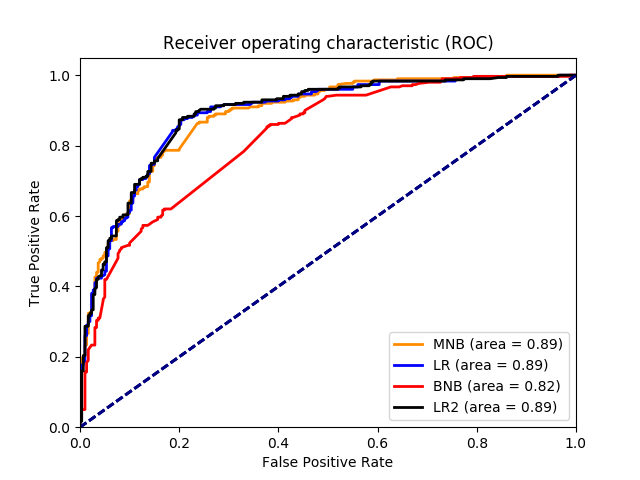
\includegraphics[scale=.5]{ROC}
		\caption{ROC curves for multinomial na\'ive Bayes, multinomial logistic regression, Bernoulli na\"ive Bayes, and logistic regression. BNB can be seen to be worse across all thresholds.}
		\label{fig:roc}
	\end{figure}
		
	\section{Discussion and Conclusion}
	
	When using feature selection, the best method was to set a low threshold for document frequency, i.e. how many times a word must appear in the whole document before it is included in the dictionary. This makes sense because we were using term frequency-inverse document frequency (tf-idf), which weights words based on their document frequency. 
	
	A useful method of feature selection was the {\bf something} score, defined as the absolute difference in occurrences of a word in positive vs. negative reviews, divided by the document frequency. 
	
	high threshold for 
	
	roc shows that logistic regression overfits less
	
	\subsubsection*{Acknowledgments}
	
	
	\bibliography{ref}
	\bibliographystyle{plain}
	
\end{document}